% ===================================================================
%  CHƯƠNG 1 - MỤC 1.2: HÀM SỐ
%  Nội dung được biên soạn lại chi tiết từ file vtp1.pdf
% ===================================================================

\section{Hàm số}
Trong toán học, một lớp ánh xạ đặc biệt quan trọng là các ánh xạ từ một tập hợp con của tập số thực vào chính tập hợp số thực. Những ánh xạ này được gọi là \textbf{hàm số thực biến số thực}, hay để ngắn gọn, chúng ta thường gọi là \textbf{hàm số}.

\begin{example}[Hàm hằng]
    Xét hàm số $f: \R \to \R$ được xác định bởi công thức $f(x) = c$, trong đó $c$ là một hằng số thực bất kỳ.
    
    Vì giá trị của hàm không thay đổi trên toàn bộ miền xác định, nó được gọi là một \textbf{hàm hằng}.
\end{example}

% -------------------------------------------------------------------
\subsection{Đồ thị}
% -------------------------------------------------------------------
Trong môn học này, chúng ta sử dụng và phát triển phương pháp \textbf{Hình học Giải tích}, một công cụ toán học nền tảng do René Descartes khởi xướng từ thế kỷ 17. Phương pháp này cho phép chúng ta:
\begin{itemize}
    \item Mô hình hóa \textbf{đường thẳng} bằng tập hợp số thực $\R$.
    \item Mô hình hóa \textbf{mặt phẳng} bằng tích của hai tập hợp số thực, $\R^2 = \R \times \R$.
\end{itemize}

Nhờ đó, các mối quan hệ phức tạp trong Hình học Euclid có thể được biểu diễn và giải quyết thông qua các phương trình và bất phương trình đại số, tạo nên một cầu nối vững chắc giữa hình học và đại số.

\begin{definition}[Đồ thị của hàm số]
    Cho một hàm số $f: D \to \R$ với miền xác định $D \subset \R$.
    
    \textbf{Đồ thị} của hàm số $f$ là tập hợp tất cả các điểm $(x, y)$ trong mặt phẳng tọa độ $\R^2$ thỏa mãn đồng thời hai điều kiện: $x \in D$ và $y = f(x)$.
    
    Ký hiệu: $G(f) = \{ (x, f(x)) \mid x \in D \}$.
\end{definition}

\begin{example}[Đồ thị hàm Parabol]
    Đồ thị của hàm số $f(x) = x^2$ với $x \in \R$ là tập hợp các điểm $\{(x, y) \in \R^2 \mid y = x^2\}$. Đây là một đường cong Parabol quen thuộc mà đỉnh của nó nằm tại gốc tọa độ.
\end{example}

Một \textbf{đường thẳng} trong mặt phẳng $\R^2$ là đồ thị của một hàm số có dạng $y = ax + b$ (đường thẳng nghiêng) hoặc là tập hợp những điểm thỏa mãn phương trình $x = c$ (đường thẳng đứng), với $a, b, c$ là các hằng số thực.

Số $a$ được gọi là \textbf{hệ số góc} (hay độ nghiêng, độ dốc) của đường thẳng. Chú ý rằng khái niệm hệ số góc không được định nghĩa cho đường thẳng đứng $x=c$.

Các hàm có dạng $y = ax + b$ vì thế đôi khi được gọi là các \textbf{hàm số tuyến tính}\footnote{Tuyến tính nghĩa là có tính thẳng. Thuật ngữ ``hàm số tuyến tính'' trong môn Vi tích phân hơi khác với thuật ngữ ``ánh xạ tuyến tính'' trong môn Đại số tuyến tính, trong môn Đại số tuyến tính thì chỉ có ánh xạ $y=ax$ mới được coi là tuyến tính.}.

Xét $(x_1, y_1)$ và $(x_2, y_2)$ là hai điểm bất kỳ trên một đường thẳng không thẳng đứng cho bởi phương trình $y = ax + b$. Vì $y_1 = ax_1 + b$ và $y_2 = ax_2 + b$ nên hệ số góc của đường thẳng này đúng bằng:
\[
a = \dfrac{(ax_2 + b) - (ax_1 + b)}{x_2 - x_1} = \dfrac{y_2 - y_1}{x_2 - x_1}
\]
Đây là công thức tính hệ số góc của một đường thẳng đi qua hai điểm cho trước. Công thức này không phụ thuộc vào cách chọn hai điểm trên đường thẳng, tương ứng với tính chất của hình học Euclid.

% Mô tả: Minh họa hệ số góc của đường thẳng không đổi, tương thích với các tam giác đồng dạng.
\begin{figure}[htbp]
    \centering
    \begin{tikzpicture}[
        scale=0.8, 
        font=\small,
        dot/.style={circle, fill, inner sep=1.2pt}
    ]
        % Load necessary libraries
        \usetikzlibrary{decorations.pathreplacing, calligraphy}

        % Vẽ hệ trục tọa độ
        \draw[->, thick] (-4.5,0) -- (4.5,0) node[below left] {$x$};
        \draw[->, thick] (0,-4) -- (0,4.5) node[below left] {$y$};

        % Vẽ đường thẳng y = 1.2x + 0.5
        \draw[thick, blue] (-3.5, -3.7) -- (3, 4.1);

        % --- Tam giác #1 (dưới cùng, bên trái) ---
        \coordinate (x1) at (-3, -3.1);
        \coordinate (x1_plus_1) at (-2, -1.9);
        \coordinate (c1) at (-2, -3.1);
        
        \draw[fill=brown!20, pattern=north east lines, pattern color=brown!60] 
            (x1) -- (x1_plus_1) -- (c1) -- cycle;
        \draw[thick] (x1) -- (x1_plus_1) -- (c1) -- cycle;
        
        \node[dot, label=left:{$(x_1, y_1)$}] at (x1) {};
        \node[dot, label=above left:{$(x_1+1, y'_1)$}] at (x1_plus_1) {};
        
        \draw[decorate, decoration={calligraphic brace, amplitude=4pt, mirror}] 
            (c1) -- (x1_plus_1) node[midway, xshift=24pt] {$y'_1 - y_1$};
        \draw[decorate, decoration={calligraphic brace, amplitude=4pt, mirror}] 
            (x1) -- (c1) node[midway, yshift=-12pt] {$1$};
        \node at ($(c1)+(-0.3,0.3)$) {};

        % --- Tam giác #3 (trên cùng, bên phải) ---
        \coordinate (x2) at (0.5, 1.1);
        \coordinate (x3) at (2.5, 3.5);
        \coordinate (c2) at (2.5, 1.1);

        \draw[fill=purple!20, pattern=north east lines, pattern color=purple!60] 
            (x2) -- (x3) -- (c2) -- cycle;
        \draw[thick] (x2) -- (x3) -- (c2) -- cycle;

        \node[dot, label=left:{$(x_2, y_2)$}] at (x2) {};
        \node[dot, label=above left:{$(x_3, y_3)$}] at (x3) {};

        \draw[decorate, decoration={calligraphic brace, amplitude=4pt, mirror}] 
            (c2) -- (x3) node[midway, xshift=24pt] {$y_3 - y_2$};
        \draw[decorate, decoration={calligraphic brace, amplitude=4pt}] 
            (c2) -- (x2) node[midway, yshift=-12pt] {$x_3 - x_2$};
        \node at ($(c2)+(-0.3,0.3)$) {};

    \end{tikzpicture}
    \caption{\centering Hệ số góc của đường thẳng không phụ thuộc vào cách chọn hai điểm để tính, tương thích với tính chất tam giác đồng dạng của hình học Euclid.}
    \label{fig:he_so_goc_v2}
\end{figure}
\begin{example}[Tính hệ số góc]
    Hệ số góc của đường thẳng nối hai điểm $(3, 5)$ và $(1, 8)$ là:
    \[
    a = \dfrac{8 - 5}{1 - 3} = \dfrac{3}{-2} = -\dfrac{3}{2}
    \]
\end{example}

Hai đường thẳng được gọi là \textbf{song song} nếu chúng khác nhau nhưng có cùng một hệ số góc hoặc cùng thẳng đứng.

\begin{example}[Ứng dụng - Chuyển đổi nhiệt độ]
    Nhiệt độ theo đơn vị Celsius ($C$) và nhiệt độ theo đơn vị Fahrenheit ($F$) có quan hệ tuyến tính với nhau. Ta biết rằng:
    \begin{itemize}
        \item $0^{\circ}C$ (nhiệt độ đông của nước) tương ứng với $32^{\circ}F$.
        \item $100^{\circ}C$ (nhiệt độ sôi của nước) tương ứng với $212^{\circ}F$.
    \end{itemize}
    Để tìm phương trình biểu diễn mối liên hệ này, chúng ta tìm phương trình của đường thẳng đi qua hai điểm $(0, 32)$ và $(100, 212)$. Hệ số góc của đường thẳng này là:
    \[
    m = \dfrac{212 - 32}{100 - 0} = \dfrac{180}{100} = \dfrac{9}{5}
    \]
    Điều này có nghĩa là khi nhiệt độ Celsius tăng $1^{\circ}$ thì nhiệt độ Fahrenheit tăng $\dfrac{9}{5}^{\circ}$.
    
    Vậy, phương trình có dạng $F = \dfrac{9}{5}C + b$. Thay điểm $(0, 32)$ vào, ta được $32 = \dfrac{9}{5}(0) + b \implies b = 32$.
    
    Công thức chuyển đổi là: $F = \dfrac{9}{5}C + 32$.
\end{example}

% -------------------------------------------------------------------
\subsection{Hàm số sơ cấp}
\label{subsec:elementary-function}
% -------------------------------------------------------------------

\subsubsection{Hàm lượng giác}
Người đọc đã học môn Lượng giác trong chương trình trung học. Tài liệu này giả sử các tính chất của các hàm lượng giác đã quen thuộc với người đọc. Dưới đây ta tóm tắt một số tính chất của hàm lượng giác mà ta thừa nhận và thường dùng.
\begin{itemize}
    \item $\sin(x)$ và $\cos(x)$ là các hàm số xác định trên $\R$, có tập giá trị trên $[-1, 1]$.
    \item $\sin(x)$ và $\cos(x)$ là các hàm tuần hoàn có chu kì là $2\pi$.
    \item $\cos(x-y) = \cos(x)\cos(y) + \sin(x)\sin(y)$.
    \item $\cos^2(x) + \sin^2(x) = 1$.
    \item Với $x \in (0, \pi/2)$ thì $\cos(x)$ là hàm giảm, $\sin(x)$ là hàm tăng.
    \item Với $x \in (0, \pi/2)$ thì $\sin x < x < \tan x$.
\end{itemize}

\noindent Từ các tính chất trên ta có thể suy ra sự tồn tại của các \textbf{hàm lượng giác ngược}:
\begin{itemize}
    \item Trên $[-\pi/2, \pi/2]$ thì hàm $\sin(x)$ là một song ánh lên $[-1, 1]$ và có hàm ngược là hàm \textbf{arcsin}.
    \item Trên $[0, \pi]$ thì hàm $\cos(x)$ là một song ánh lên $[-1, 1]$ và có hàm ngược là hàm \textbf{arccos}.
    \item Trên $(-\pi/2, \pi/2)$ thì hàm $\tan(x)$ là một song ánh lên $\R$ và có hàm ngược là hàm \textbf{arctan}.
\end{itemize}

\subsubsection{Hàm lũy thừa và hàm mũ}

Với $x$ là một số thực khác 0, nếu $n$ là một số nguyên dương thì $x^n$ là tích của $n$ số $x$. Nếu $n$ là một số nguyên âm thì ta định nghĩa $x^n$ là số thực $\dfrac{1}{x^{-n}}$. Ta định nghĩa $x^0=1$.

Nếu $x > 0$ và $n$ là một số nguyên dương thì có duy nhất một số thực không âm $a$ sao cho $a^n = x$. Có thể chứng tỏ điều này bằng cách dùng tính đầy đủ của tập hợp số thực. Số $a$ được gọi là căn bậc $n$ của $x$, kí hiệu là $\sqrt[n]{x}$ hay $x^{\frac{1}{n}}$.

Nếu $x > 0$ và $m \in \Z$, $n \in \Z^+$ thì $x^{\frac{m}{n}}$ được định nghĩa là $\sqrt[n]{x^m}$.

Như vậy khi $x > 0$ và $r \in \Q$ thì $x^r$ đã được định nghĩa. Khi $r \in \R$ thì định nghĩa cần thông qua quá trình giới hạn, từ việc xấp xỉ số thực bởi số hữu tỉ.

\begin{example}
    Có thể định nghĩa $2^{\pi}$ bằng cách lấy một dãy số hữu tỉ dương $r_n$ hội tụ về $\pi$ (ví dụ: $3, 3.1, 3.14, 3.141, \dots$) rồi đặt $2^{\pi} = \limit{n}{\infty} 2^{r_n}$.
\end{example}

\begin{definition}(Hàm lũy thừa, hàm mũ) Từ những ý trên, ta có định nghĩa như sau (Hình ~\ref{fig:plot_exp_functions}):
    \begin{itemize}
        \item Với $r \in \R$ cho trước thì hàm $f(x) = x^r$ được gọi là một \textbf{hàm lũy thừa}.
        \item Với $a > 0$ và $a \ne 1$ cho trước thì hàm $f(x) = a^x$ được gọi là một \textbf{hàm mũ}.
    \end{itemize}
\end{definition}

% Minh họa một số hàm mũ thường gặp
\begin{figure}[htbp]
    \centering
    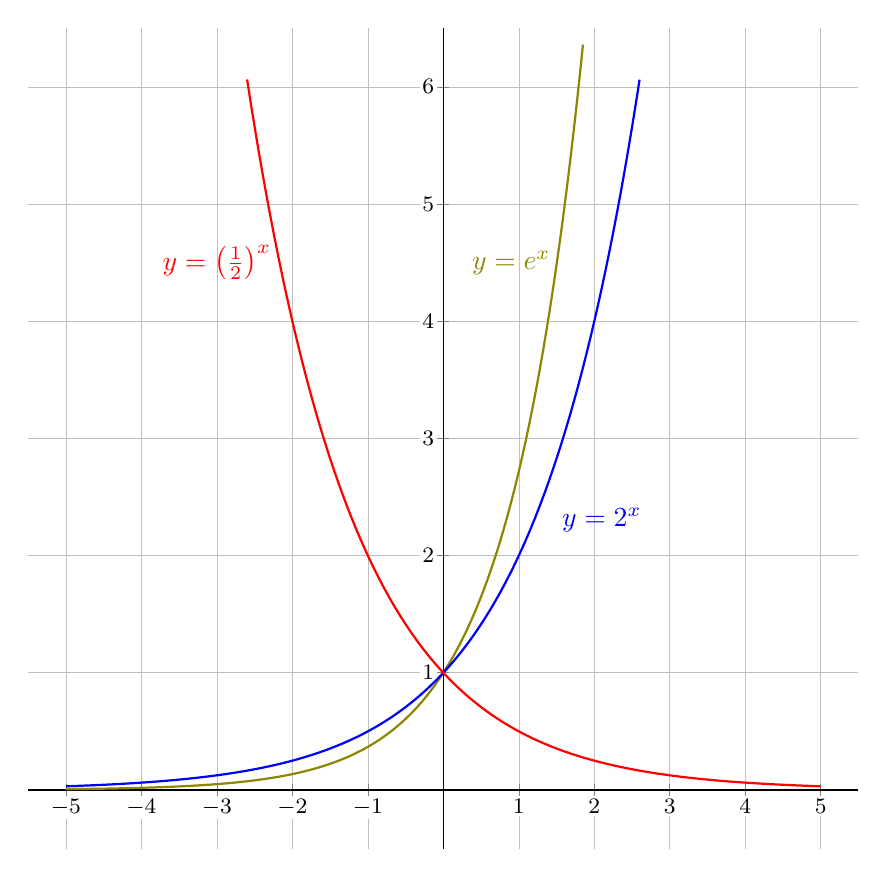
\begin{tikzpicture}
        % --- (giữ nguyên code vẽ hình của bạn ở đây) ---
        \begin{axis}[
            width=1\textwidth,
            height=12cm,
            axis lines=middle,
            grid=major,
            grid style={line width=.1pt, draw=gray!20},
            major grid style={line width=.2pt,draw=gray!50},
            xmin=-5.5, xmax=5.5,
            ymin=-0.5, ymax=6.5,
            xtick={-5, -4, -3, -2, -1, 0, 1, 2, 3, 4, 5},
            ytick={1, 2, 3, 4, 5, 6},
            ticklabel style={font=\footnotesize, fill=white, inner sep=1pt},
            axis line style={-},
            smooth,
            no marks,
            samples=200,
        ]

        % Vẽ đồ thị y = e^x
        \addplot[olive, thick, domain=-5:1.85] {exp(x)}; % Đổi màu blackgreen thành olive cho chuẩn
        \node[olive] at (axis cs:0.9, 4.5) {$y=e^x$};

        % Vẽ đồ thị y = 2^x
        \addplot[blue, thick, domain=-5:2.6] {2^x};
        \node[blue] at (axis cs:2.1, 2.3) {$y=2^x$};

        % Vẽ đồ thị y = (1/2)^x
        \addplot[red, thick, domain=-2.6:5] {(1/2)^x};
        \node[red] at (axis cs:-3, 4.5) {$y=\left(\frac{1}{2}\right)^x$};

        \end{axis}
    \end{tikzpicture}
    \caption{Đồ thị của một số hàm mũ.\footnotemark} % <-- SỬA Ở ĐÂY: Dùng \footnotemark
    \label{fig:plot_exp_functions}
\end{figure}
\footnotetext{Chú ý dáng điệu và sự khác nhau khi cơ số lớn hơn 1 và bé hơn 1.} % <-- SỬA Ở ĐÂY: Dùng \footnotetext ngay sau figure

Hàm mũ $a^x$ có hàm ngược là \textbf{hàm lô-ga-rít cơ số a}\footnote{tiếng Anh là logarithm}, kí hiệu là $\log_a$. Như vậy
\[ y = a^x \iff x = \log_a y. \]

\begin{proposition}
    (Một số công thức cho hàm logarithm)
    \begin{itemize}
        \item $log_a(bc) = log_a(b) + log_a(c)$
        \item $log_a(\dfrac{b}{c}) = log_a(b) - log_a(c)$
        \item $log_a(b^{\alpha}) = \alpha \cdot log_a(b)$
        \item $log_{a^{\alpha}}(b) = \dfrac{1}{\alpha} \cdot log_a(b) $
        \item $log_a(b) = \dfrac{1}{log_b(a)}$
        \item $a^{log_a(b)} = b$
        \item $log_a(c) = log_a(b) \cdot log_b(c)$
        \item $a^{log_b(c)} = c^{log_a(b)}$
    \end{itemize}
\end{proposition}

\begin{example}[Mô hình lãi kép]
    Giả sử một khoản tiền $A_0$ được gửi vào một tài khoản ngân hàng với lãi suất $r$ cho mỗi kỳ hạn. Tại thời điểm ban đầu $t=0$, số tiền là $A(0) = A_0$. Sau mỗi kỳ hạn, tiền lãi được nhập vào vốn để tính lãi cho kỳ tiếp theo. Đây được gọi là \textbf{lãi nhập vốn} (hay lãi kép). Ta muốn biết tại thời điểm $t$ (sau $t$ kỳ hạn) thì giá trị của khoản tiền là bao nhiêu?
    \begin{itemize}
        \item Sau 1 kỳ hạn: $A(1) = A(0) + A(0)r = A(0)(1+r)$.
        \item Sau 2 kỳ hạn: $A(2) = A(1) + A(1)r = A(1)(1+r) = A(0)(1+r)^2$.
        \item Sau 3 kỳ hạn: $A(3) = A(2) + A(2)r = A(2)(1+r) = A(0)(1+r)^3$.
    \end{itemize}
    Đến đây ta có thể dự đoán công thức giá trị của $A$ sau $t$ kỳ hạn chính là
    \[ A(t) = A(0)(1+r)^t. \]
    Các tính toán trên cho thấy ta có thể dễ dàng kiểm tra công thức này là đúng bằng phương pháp quy nạp toán học.
\end{example}

Hằng số $e$ là một số thực thường gặp, là một số vô tỉ, biểu diễn thập phân có các chữ số đầu là $2,71828\dots$\footnote{Kí hiệu $e$ có thể có nguồn gốc từ tên Euler (một trong những người đầu tiên sử dụng số này), hoặc exponent (mũ), và còn được gọi là hằng số Napier (tên Napier còn được viết là Néper).}. Hằng số này có thể được định nghĩa là giới hạn của một dãy số hữu tỉ bằng công thức
\[ e = \limit{n}{\infty} \left(1 + \dfrac{1}{n}\right)^n. \]

Hàm mũ $y=e^x$ có hàm ngược được gọi là \textbf{hàm lô-ga-rít tự nhiên}\footnote{trong tiếng Anh là natural logarithm. Chú ý một số tài liệu và phần mềm lại dùng kí hiệu `log' để chỉ hàm lô-ga-rít tự nhiên.} \footnote{các công thức cho hàm logarithm vẫn đúng cho hàm natural logarithm}, kí hiệu là $\ln$. Vậy
\[ y = e^x \iff x = \ln y. ~\ref{fig:plot_e^x_ln(x)}\]

% Hình minh họa cho sự đối xứng của 2 hàm
\begin{figure}[H] % Để canh giữa và thêm chú thích
    \centering % Canh giữa hình
    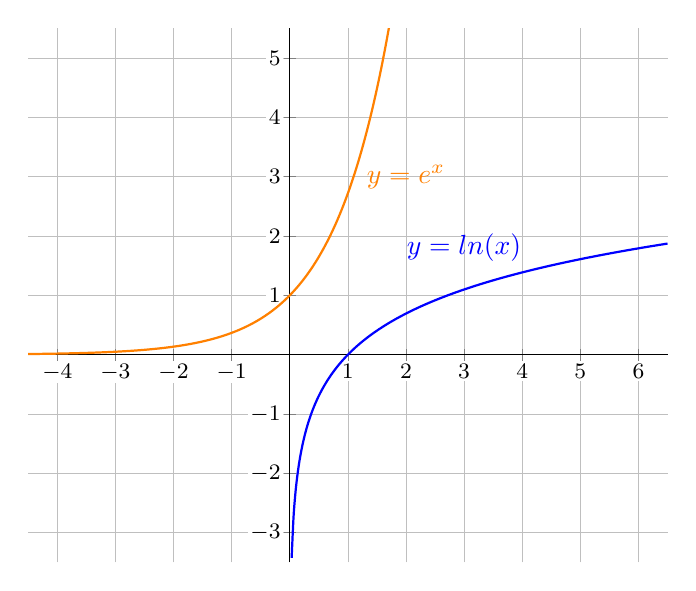
\begin{tikzpicture}
        \begin{axis}[
            width=0.8\textwidth,
            % height=12cm,
            axis lines=middle,
            grid=major,
            grid style={line width=.1pt, draw=gray!20},
            major grid style={line width=.2pt,draw=gray!50},
            xmin=-4.5, xmax=6.5,
            ymin=-3.5, ymax=5.5,
            xtick={-4, -3, -2, -1, 0, 1, 2, 3, 4, 5, 6},
            ytick={-3, -2, -1, 0, 1, 2, 3, 4, 5, 6},
            ticklabel style={font=\footnotesize, fill=white, inner sep=1pt},
            axis line style={-},
            smooth,
            no marks,
            samples=200,
        ]

        % Vẽ đồ thị y = e^x
        \addplot[orange, thick, domain=-5:1.85] {exp(x)};
        \node[orange] at (axis cs:2, 3) {$y=e^x$};

        % Vẽ đồ thị y = ln(x)
        \addplot[blue, thick, domain=0:6.5] {ln(x)};
        \node[blue] at (axis cs:3, 1.8) {$y=ln(x)$};

        \end{axis}
    \end{tikzpicture}
    \caption{Đồ thị các hàm số $y = e^x$ và $y = ln(x)$.} % Thêm chú thích cho hình (tùy chọn)
    \label{fig:plot_e^x_ln(x)} % Thêm nhãn để tham chiếu (tùy chọn)
\end{figure}

Tổng, hiệu, tích, thương, hàm hợp của các hàm lũy thừa, hàm mũ, hàm log, hàm lượng giác, hàm lượng giác ngược được gọi là các \textbf{hàm số sơ cấp}. Trong các hàm sơ cấp có các hàm thường gặp như hàm đa thức, hàm phân thức (thương của hai đa thức), hàm căn thức.

\begin{example}
    Hàm mũ $f(x) = e^x$ cùng với hàm $g(x) = \cos x$ cho hàm hợp $(f \circ g)(x) = f(g(x)) = e^{\cos x}$ và $(g \circ f)(x) = g(f(x)) = \cos(e^x)$. Đây là những hàm sơ cấp.
\end{example}

\subsection{Bài tập}

\begin{exercise}
Viết phương trình đường thẳng có các tính chất sau đây:
    \begin{enumerate}[label=(\alph*)]
        \item Có hệ số góc là 2 và giao với trục Oy tại $(0,3)$.
        \item Đi qua các điểm $(2,3)$ và $(4,5)$.
        \item Đi qua điểm $(2,1)$ và song song với đường thẳng $y = -4x + 3$.
    \end{enumerate}
\end{exercise}

\begin{exercise}
Giải các phương trình sau:
    \begin{enumerate}[label=(\alph*)]
        \item $3e^{2x-4} = 5$.
        \item $-1 + 2\ln(2 - 3x) = 9$.
    \end{enumerate}
\end{exercise}

\begin{exercise}
Một người gửi 3 triệu đồng vào một tài khoản tiết kiệm với lãi suất 6\% một năm, kì hạn (thời điểm tính lãi gộp vốn) là 1 năm.
    \begin{enumerate}[label=(\alph*)]
        \item Sau 4 năm thì tài khoản có bao nhiêu tiền?
        \item Bao lâu thì người đó có được 10 triệu đồng?
    \end{enumerate}
\end{exercise}

\begin{exercise}
Năm 2024, GDP của Việt Nam là 476 tỉ USD (đứng thứ 33 trên thế giới) với tốc độ tăng trưởng là 7,1\% mỗi năm. Cùng năm, GDP của Thái Lan là 526 tỉ USD với tốc độ tăng trưởng là 2,5\% mỗi năm.\footnote{theo \href{https://datatopics.worldbank.org/world-development-indicators/themes/economy.html}{worldbank - 2024}} Giả sử hai tốc độ tăng trưởng này được giữ nguyên trong tương lai.
    \begin{enumerate}[label=(\alph*)]
        \item Khi nào thì GDP của Việt Nam đạt GDP của Thái Lan năm 2024?
        \item Khi nào thì GDP của Việt Nam đuổi kịp GDP của Thái Lan?
    \end{enumerate}
\end{exercise}

%-------------------------------------------------
% CÁC BÀI TẬP MỚI ĐƯỢC TẠO RA
%-------------------------------------------------

\begin{exercise}
Sử dụng các tính chất của logarit để rút gọn biểu thức sau mà không dùng máy tính:
$$ A = \log_2(80) + \log_2(6) - \log_2(15) $$
\end{exercise}

\begin{exercise}
Tìm hàm số ngược $f^{-1}(x)$ của hàm số sau:
$$ f(x) = e^{2x} + 3 $$
\end{exercise}

\begin{exercise}
Đồng vị Carbon-14 ($^{14}C$) có chu kỳ bán rã là 5730 năm. Một mẫu vật khảo cổ được tìm thấy có lượng $^{14}C$ chỉ bằng 30\% so với lượng $^{14}C$ trong một cơ thể sống. Hãy ước tính tuổi của mẫu vật này.\footnote{xem thêm cơ chế hoạt động tại \href{https://vi.wikipedia.org}{wikipedia - Định tuổi bằng $^{14}C$}}
\end{exercise}

\begin{exercise}
Cho đồ thị của hàm số $y = \ln(x)$. Hãy mô tả các phép biến đổi (tịnh tiến, đối xứng) cần thực hiện để thu được đồ thị của hàm số:
$$ y = -\ln(x+2) $$
\end{exercise}

\begin{exercise}
``Luật Moore là một quan sát và dự đoán do Gordon Moore, đồng sáng lập Intel, đưa ra. Một phiên bản phổ biến của luật này phát biểu rằng: \textit{``Số lượng transistor trên một vi mạch tích hợp sẽ tăng gấp đôi sau mỗi hai năm."}

Điều này cũng có nghĩa là kích thước của các transistor sẽ ngày càng thu nhỏ. Dữ liệu thực tế cho thấy kích thước transistor trong các bộ xử lí máy tính là \textbf{14\,nm} (nanometer) vào năm 2014 và giảm xuống còn \textbf{10\,nm} vào năm 2016.

\begin{enumerate}[label=(\alph*)]
    \item Hãy giải thích vì sao dữ liệu trên là phù hợp với Định luật Moore.
    
    \item Dựa vào xu hướng này, hãy xây dựng một mô hình hàm số mũ $S(t) = S_0 \cdot a^t$ để mô tả sự thay đổi của kích thước transistor theo thời gian $t$ (tính bằng năm, với $t=0$ là năm 2014). Sau đó, hãy dùng mô hình này để dự đoán vào năm nào quy trình sản xuất có thể đạt được kích thước transistor là \textbf{5\,nm}\footnote{bạn đọc có thể đối chứng kết quả tại: \href{https://en.m.wikipedia.org/wiki/5_nm_process}{wikipedia - 5nm-transistor}}.
\end{enumerate}
\end{exercise}